\documentclass[a4paper,11pt]{article}

\usepackage{graphicx}
\usepackage[sort&compress]{natbib}
\usepackage{pdfpages}
\usepackage{amsmath}
\usepackage{breqn}
\usepackage{amssymb}
\usepackage{float}
\usepackage{listings}
\usepackage[a4paper]{geometry}
\usepackage{hhline}
\usepackage{makecell}
\usepackage{amsthm}
\usepackage{caption}
\usepackage{subcaption}
\usepackage{hyperref}
\usepackage{tikz}
\graphicspath{{./figures/}}

\begin{document}

\theoremstyle{plain}
\newtheorem{thm}{Theorem}{}

\theoremstyle{definition}
\newtheorem{defn}[thm]{Definition}

\renewcommand{\vec}[1]{\mathbf{#1}}

\title{Research Project Proposal - Finding Interesting Patterns in Workflow Logging Data}
\date{\today}
\author{
        Dani\"el Stekelenburg		
}
 
% TO ADD:
% 1. Extend word2vec with problems and possible solutions
% 2. Propose to do an approach without the application of word2vec. This to verify that the other algorithms (like inductive miner) are effective.
% 3. Discuss (the difficulty of) defining when a given process tree (pattern) is contained within another process tree. (induced/embedded subtrees???)  
% 4. Include word2vec model in the complete approach.
% 5. Say something about conformance checking...
 
\maketitle

\abstract{}

% \subsection{The word2vec model}
% \label{section:word2vec}
% The model is proposed in 2013 by \cite{Mikolov2013a,Mikolov2013b}. The earlier work of Mikolov et al. \cite{Mikolov2013a} explains the use of a continuous-bag-of-words model (CBOW). A bag-of-words model translates a given document as a bag of words. Since word2vec uses the notion of neural networks, let me explain this concept shortly. 

% \subsubsection{Neural Networks}
% An artificial neural network is based on a biological phenomenom, the human brain. Like a human brain, a neural network exists of neurons. Depending on the given information, i.e. input values, the neurons give a certain output. The input values and their weights can also be represented as vectors $\vec{x}$ and $\vec{w}$. For a more graphical example, see Figure \ref{figure:neuron}.

% The input of a neuron is determined by computing average of the sum over the input values and their weights, defined as 

% \begin{equation}
% u = \sum_{i=0}^{K}w_i x_i = \vec{w}^T \vec{x}.
% \end{equation}

% A neuron uses a function $f(u)$ to determine its output value. For instance, you can use a simple function like the binary threshold-function:

% \begin{equation}
% f(u) = \begin{cases}
% 1 & \vec{w}^T \vec{x} \geq \theta \\
% 0 & \text{otherwise}
% \end{cases}
% \end{equation}
% Using this function, a neuron results in either a 1 or a 0. However, there are also more complex functions from which the number of possible output values is much higher, resulting in a more detailed network. But the important thing to know is, that a layer of neurons influence the next layer etc. Eventually, in the output layer, the neuron with the highest value is the classified answer of the network.

% Neurons have three different types, input, hidden and output. Figure \ref{figure:neuralnetwork} presents a multi-layered neural network (note the three layers). Neurons in the input layer already have a certain value, whereas the hidden needs to compute its output values for every neuron in the next layer. Ultimately, the output layer consists of neurons representing the possible answers you are looking for. 

% \begin{figure}[h]
% \begin{subfigure}{.5\textwidth}
%   \centering
%   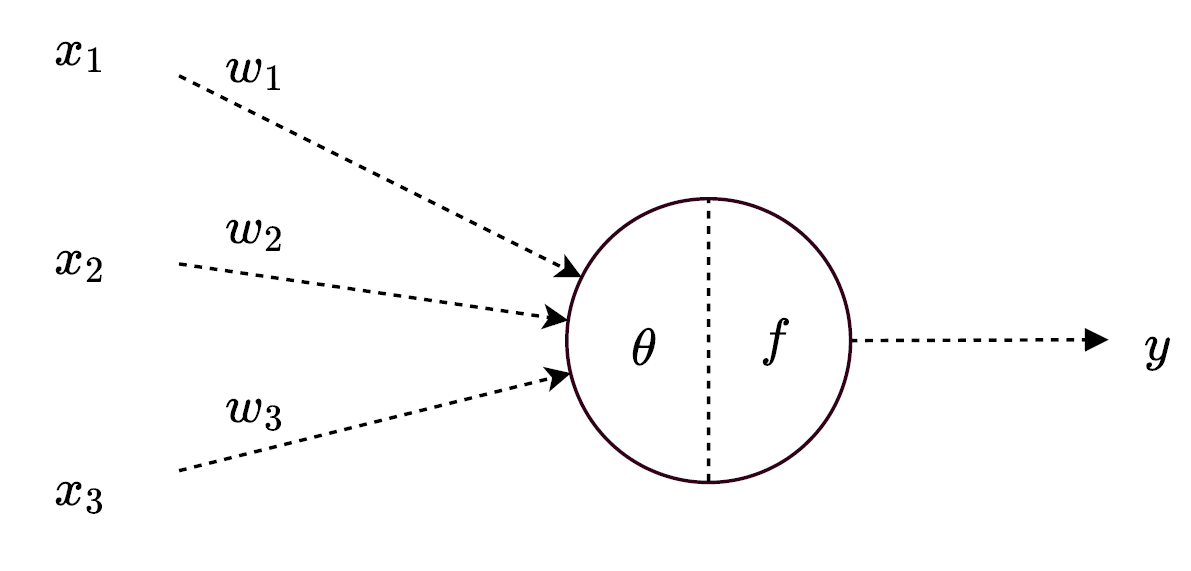
\includegraphics[width=.8\linewidth]{Neuron.png}
%   \caption{A neuron.}
%   \label{figure:neuron}
% \end{subfigure}%
% \begin{subfigure}{.6\textwidth}
%   \centering
%   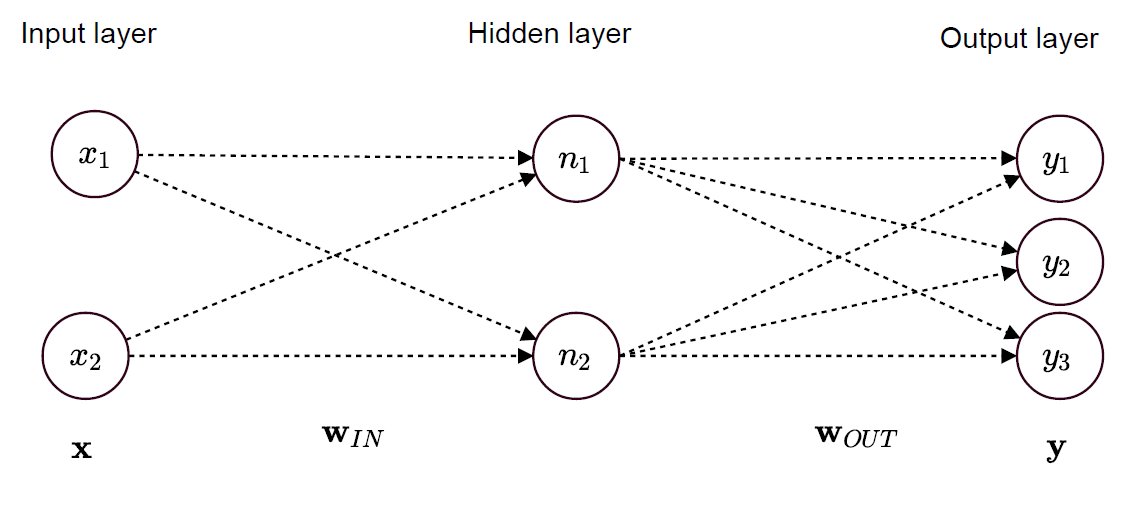
\includegraphics[width=.9\linewidth]{NeuralNetworkExample.png}
%   \caption{Example of a neural network.}
%   \label{figure:neuralnetwork}
% \end{subfigure}
% \caption{On the left, see the basic environment of a neuron. On the right, a multi-layered neural network is shown.}
% \label{figure:NeuralNetworks}
% \end{figure}

% \subsubsection{Continuous Bag-of-Words Model}
% The Continuous bag-of-words model \cite{Mikolov2013a} is the first part of the word2vec technique. This model uses context words as its input and, using a neural network, outputs the target word for which the model thinks is the most likely word with the context words as its surrounding. The simplest version of this model is a model which uses one context word, as shown in Figure \ref{figure:one-context-word}. Here, the vector $\vec{x}$ is a one-hot vector, meaning that it only contains a $1$ once and the rest of the $V$ positions are $0$'s. The size $V$ depends on the number of words used in the dictionary, and every word has a different vector $\vec{x}$.

% The weights are represented by the matrices $\vec{W}_{V \times N}$ and $\vec{W'}_{N \times V}$, where every row $i$ in $\vec{W}_{V \times N}$ represents the weights vector $\vec{w}^T_i$ (with length $N$) for a context word. Thus, given a context word $w_A$, where $x = [0\ldots,0,1,0\ldots0]^T$ assuming $x_k=1$ and $x_k'=0$ for $x_k' \not= x_k$, the hidden layer will become $\vec{h}$ like,

% \begin{equation}
% \vec{h} = \vec{W}^T\vec{x} = \vec{W}^T_{(k,\cdot)} = \vec{v}^T_{w_k}
% \end{equation}

% In other words, we copy the $k$-th row of $\vec{W}$ to $\vec{h}$, which we simply call $\vec{v}^T_{w_k}$. For the output, we use matrix $\vec{W'}_{N \times V}$, which contains the weights of each $N$-sized representation of the hidden layer in order to compute the output layer. Note that the output layer, like the input layer, has the same number of neurons ($V$ in our case). This is quite obvious, since $V$ represents the number of words we can use and we are looking for a word. Computing this target word is done by computing a score $u_j$ for each possible word, like
% \begin{equation}
% u_j = \vec{v'}_{w_j}^T \vec{h},
% \end{equation}
% where $\vec{v'}_{w_j}^T$ is the $j$-th column in the matrix $\vec{W'}$. After every $u_j$ for every $j \in [1-V]$ are computed, the value for each value $y_j$ $\vec{y}$ is determined using a softmax function for normalization \cite{bishop2007pattern}:

% \begin{equation}
% y_j = p(w_j|w_A) = \dfrac{\exp(u_j)}{\sum_{j'=1}^V \exp(u_j')}.
% \end{equation}
% Here, $p(w_j|w_A)$ stands for the probability of the word $w_j$ being the target word, considering the context word $w_A$. Eventually, the highest value $y_j$ is the predicted answer of your query. The goal of training this model is to maximize the value $y_j$ for the label $w_O$, which we want to predict. The loss function $E=-log \textit{p}(w_O|w_I)$ represents the error made by the model (we try to minimize $E$). Having a perfect prediction results in $E=0$. Updating this model is done using this loss function.

% \begin{figure}[H]
% \centering
% 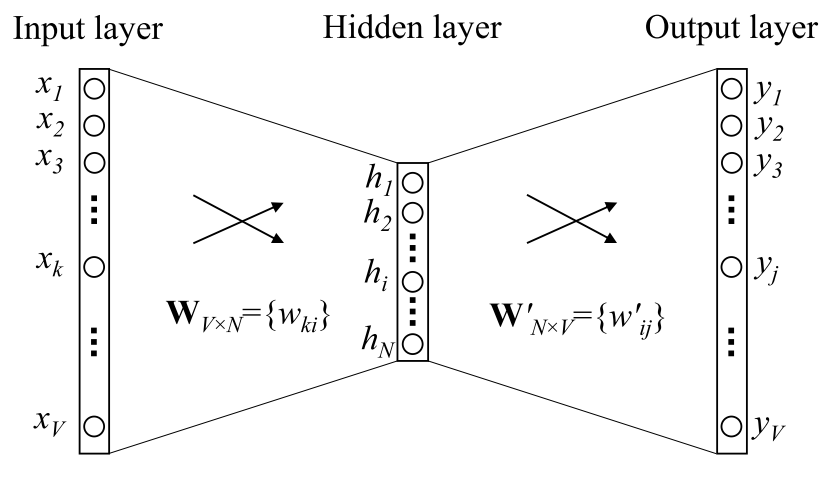
\includegraphics[width=.7\linewidth]{one-context-word.png}
% \caption{CBOW model which uses only one context word as input. Source: \cite{Rong2014word2vec}}
% \label{figure:one-context-word}
% \end{figure}

% % Explain updating the weights...

% \subsubsection{Skip-gram Model}
% Whereas the context words are the input of the CBOW model, the Skip-gram model \cite{Mikolov2013b} uses the target word as its input and gives the context words as output. Simply put, the skip-gram model works the other way around.

% \begin{figure}[H]
% \centering
% 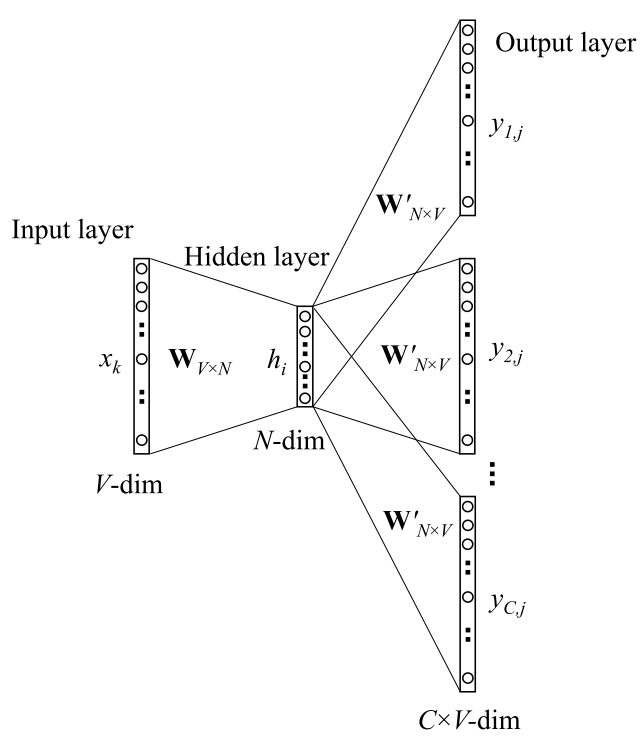
\includegraphics[width=.6\linewidth]{skip_gram.png}
% \caption{The skip-gram model. Source: \cite{Rong2014word2vec}}
% \label{figure:skip-gram}
% \end{figure}


\bibliographystyle{unsrt}
\bibliography{sources}

\end{document}